\documentclass{article}
\usepackage{CJK}
\usepackage{ctex}
\usepackage{graphicx}
\usepackage{float}
\usepackage[colorlinks,linkcolor=black]{hyperref}
\graphicspath{{pic/}}
\renewcommand{\contentsname}{目录}
\renewcommand{\abstractname}{摘要}
\title{MusiCube - 手势音游\\
       项目中期报告}
\author{杨铭 - 5130379022\\
        李晟 - 5130379017\\
        张云翔 - 5130379012}
\begin{document}
\maketitle
\tableofcontents
\newpage
\section{项目概述}
\paragraph{}
电子游戏,被认为是第九大艺术,在电子产品和网络愈发普及的今天,被越来越多的人所承认和喜爱。而作为游戏中一种独特的类型——音乐游戏(MUG),由最早的街机发展而来,因其与音乐的结合,受到不少玩家的喜爱。
\paragraph{}
而随着VR,AR等概念的兴起,电子游戏的玩法也将出现新的变革。MusiCube就是一款突破性的音乐游戏,它使用了不同于之前音乐游戏键盘,鼠标或是手台的输入方式,利用LeapMotion的手势识别,让玩家可以更加自由地感受音乐游戏的快感。
\paragraph{}
在MusiCube中,所用的音符节拍将都在一个立体的魔方上出现,玩家可以通过手部的动作来操作魔方表面的音符,如戳击一个块,旋转一层。不仅如此,我们还提供图谱编辑器,玩家可以自由编辑自己的图谱,将来如果可能,还可以建立玩家社区,集排名,作图,讨论,自定义皮肤等功能于一体,丰富游戏的玩法,提升游戏的深度,增加玩家的粘性。
\begin{figure}[H]
  % Requires \usepackage{graphicx}
  \begin{minipage}{0.5\linewidth}
    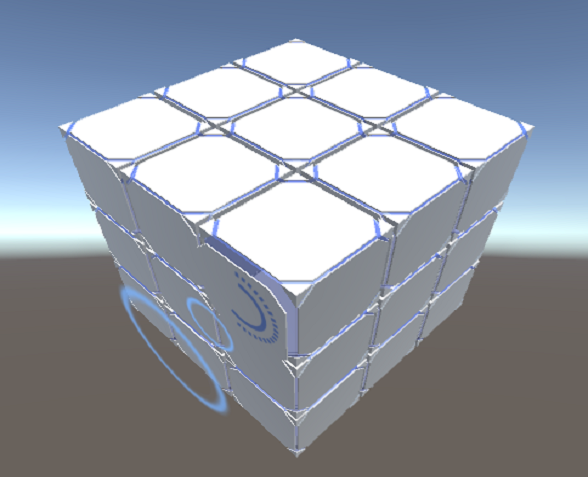
\includegraphics[width=15em]{mid-demo1.png}\\
    \caption{}\label{demo1}
  \end{minipage}
  \begin{minipage}{0.5\linewidth}
    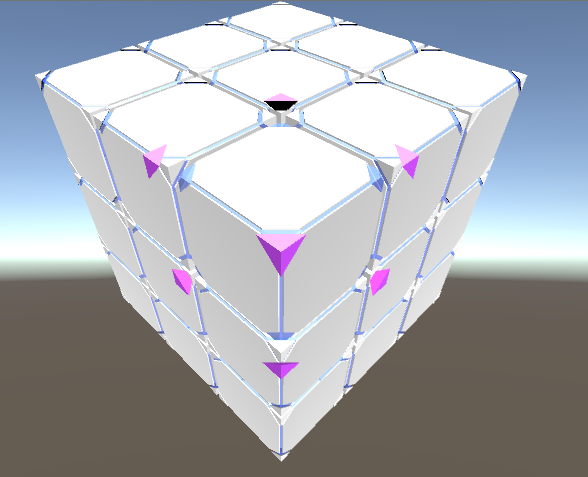
\includegraphics[width=15em]{mid-demo2.png}\\
    \caption{}\label{demo2}
  \end{minipage}
\end{figure}
\begin{description}
  \item[软件类型] 游戏 - 音乐游戏(MUG)
  \item[目标用户] PC用户、游戏玩家
  \item[平台支持] PC - Windows7及以上版本
  \item[硬件支持] LeapMotion
\end{description}
\newpage
\section{需求分析}
\subsection{用户分析}
我们主要针对青少年做了问卷调查
\paragraph{对音乐游戏的熟悉程度}
\begin{figure}[H]
  \centering
  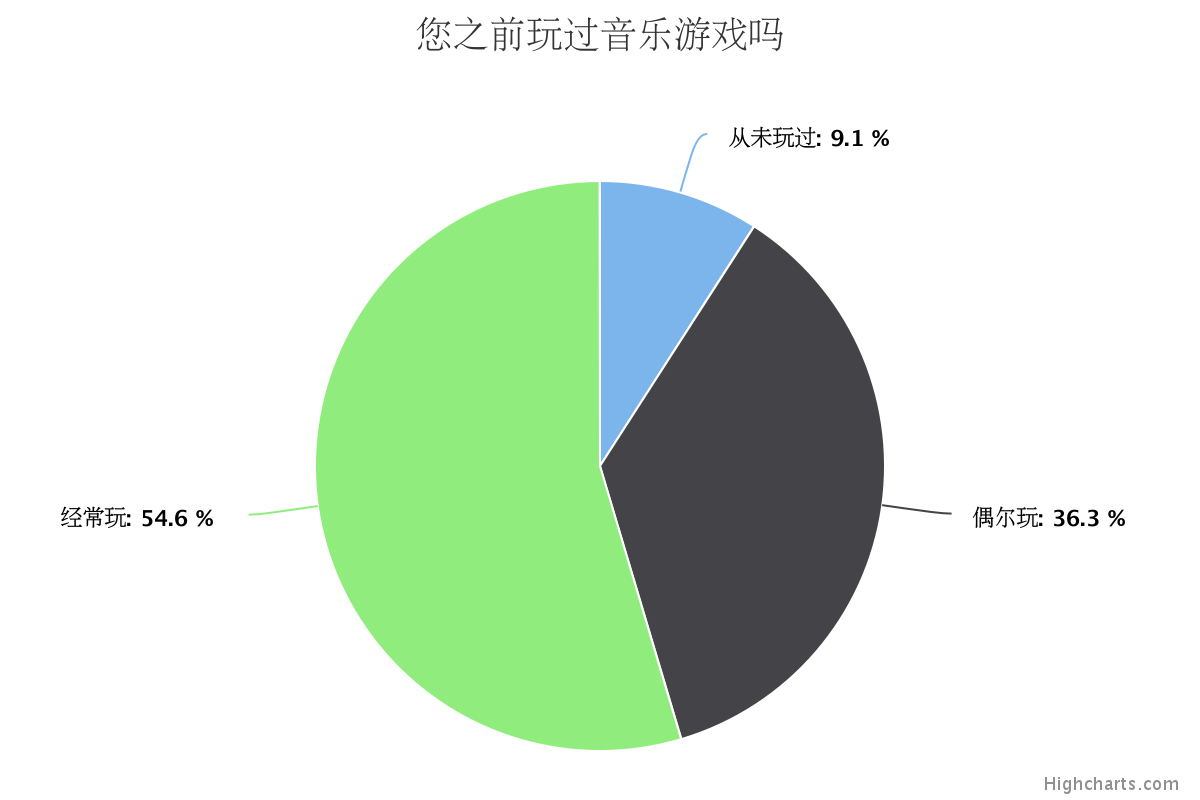
\includegraphics[width=22em]{chart1.png}\\
  \caption{您之前玩过音乐游戏吗}\label{2-1}
\end{figure}
\paragraph{}
由于在调查时,一些人表示不熟悉音乐游戏而拒绝了填写问卷,并且调查时间较短,所以推测数据有一定偏差。但从目前的数据来看,大多青少年和大学生都
玩过音乐游戏,一大半的人经常玩音乐游戏,可以看出音乐游戏的市场还是较为广阔。
\paragraph{玩音乐游戏的平台}
\begin{figure}[H]
  \centering
  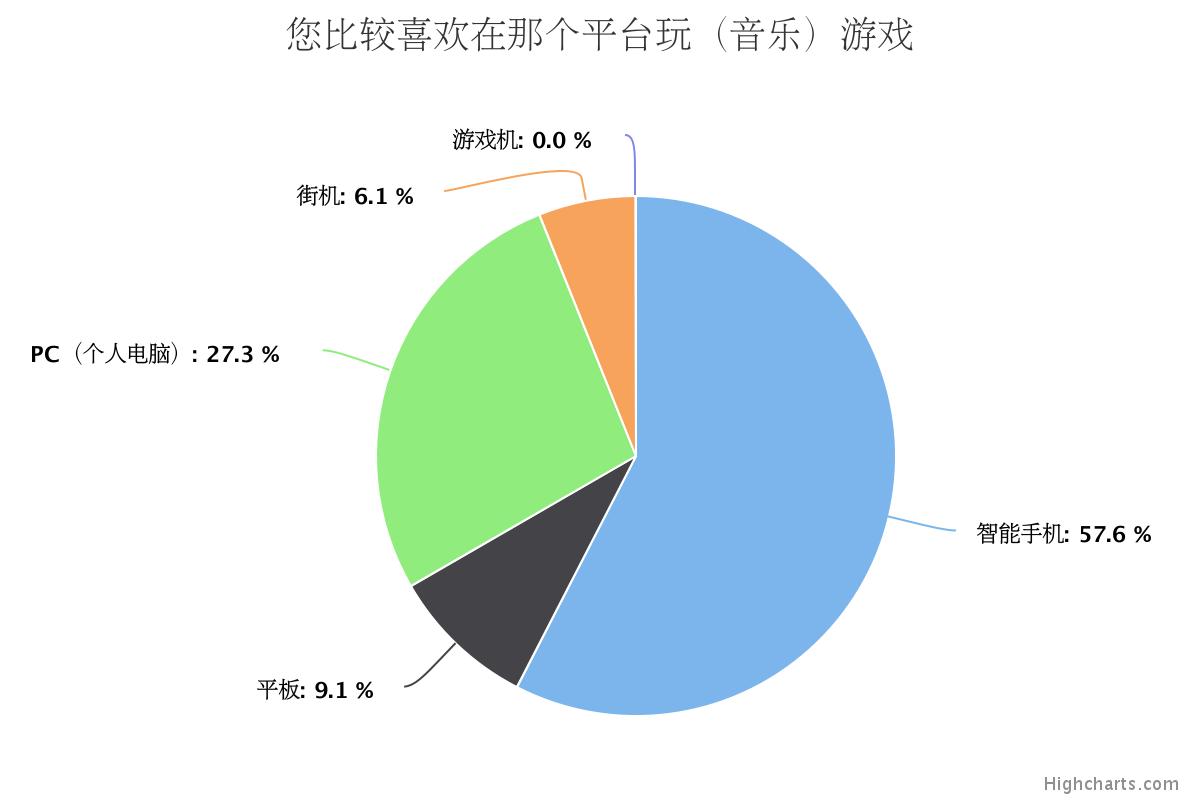
\includegraphics[width=22em]{chart2.png}\\
  \caption{您一般在那个平台玩(音乐)游戏}\label{2-2}
\end{figure}
\paragraph{}
随着智能手机的兴起,大家的娱乐时间日渐碎片化,从调查结果中也可见一斑。现在也有许多音乐游戏厂商在向智能手机或平板等移动设备进军,如:在日本火爆的LoveLive、腾讯的节奏大师、雷亚的deemo和在内测中的VOEZ。
但是不可否认的是PC端仍是许多玩家特别是精英玩家的必选平台,为音乐游戏,作为一种注重培养精英玩家的游戏,快餐式的游戏体验不能给玩家带来许多乐趣。因为音乐游戏需要快速反应和对音乐的熟悉来获取更好的成绩,
想要提高水准,一般只能用圈内所说的“堆PC”,也就是多次尝试来达成。而愿意花费大量时间的玩家往往不会在乎平台的区别,所以我们认为PC客户端的Musicube在音游圈仍旧有不错的市场。
\paragraph{虚拟现实}
\begin{figure}[H]
  \centering
  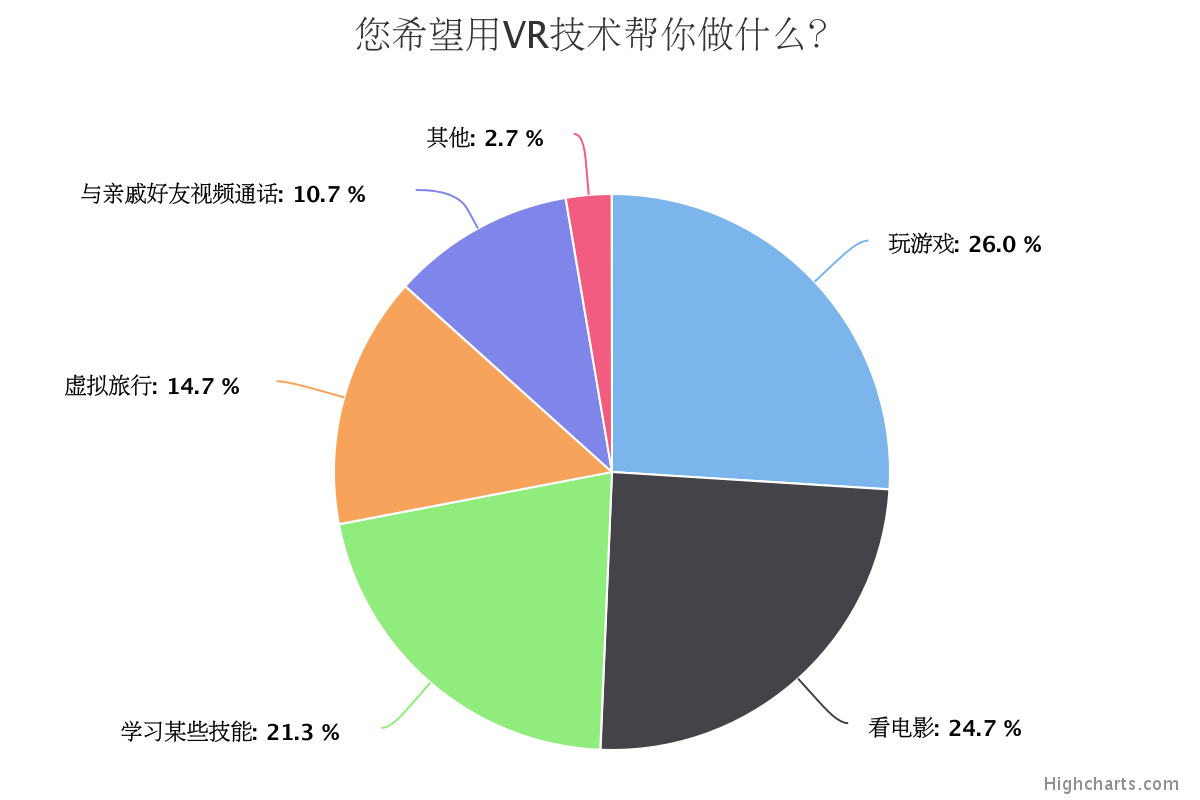
\includegraphics[width=22em]{chart.png}\\
  \caption{您希望VR技术帮你做什么}\label{2-3}
\end{figure}
\paragraph{}
从调查中可以看出,大多数用户对虚拟现实技术的期望,还是在家庭娱乐方面:选择玩游戏,看电影的接近一半。在键盘鼠标显示器等传统输入输出设备统治电子娱乐几十年以后,新兴的VR设备是否能够颠覆这一行业仍需观察,
但至少在许多使用者看来,是时候有些改变了。
\begin{figure}[H]
  \centering
  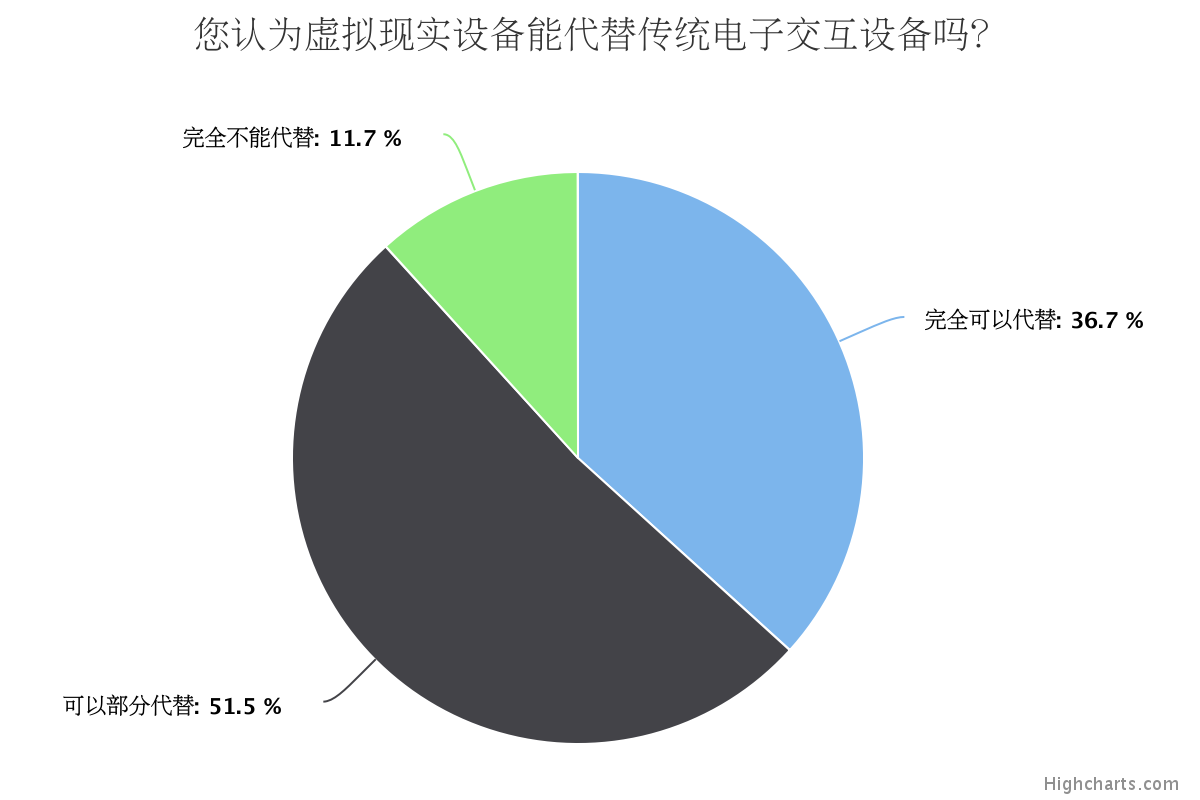
\includegraphics[width=22em]{chart6.png}\\
  \caption{对VR设备的期望}\label{2-4}
\end{figure}
\newpage
\paragraph{您觉得用手势玩音乐游戏怎么样}
\begin{figure}[H]
  \centering
  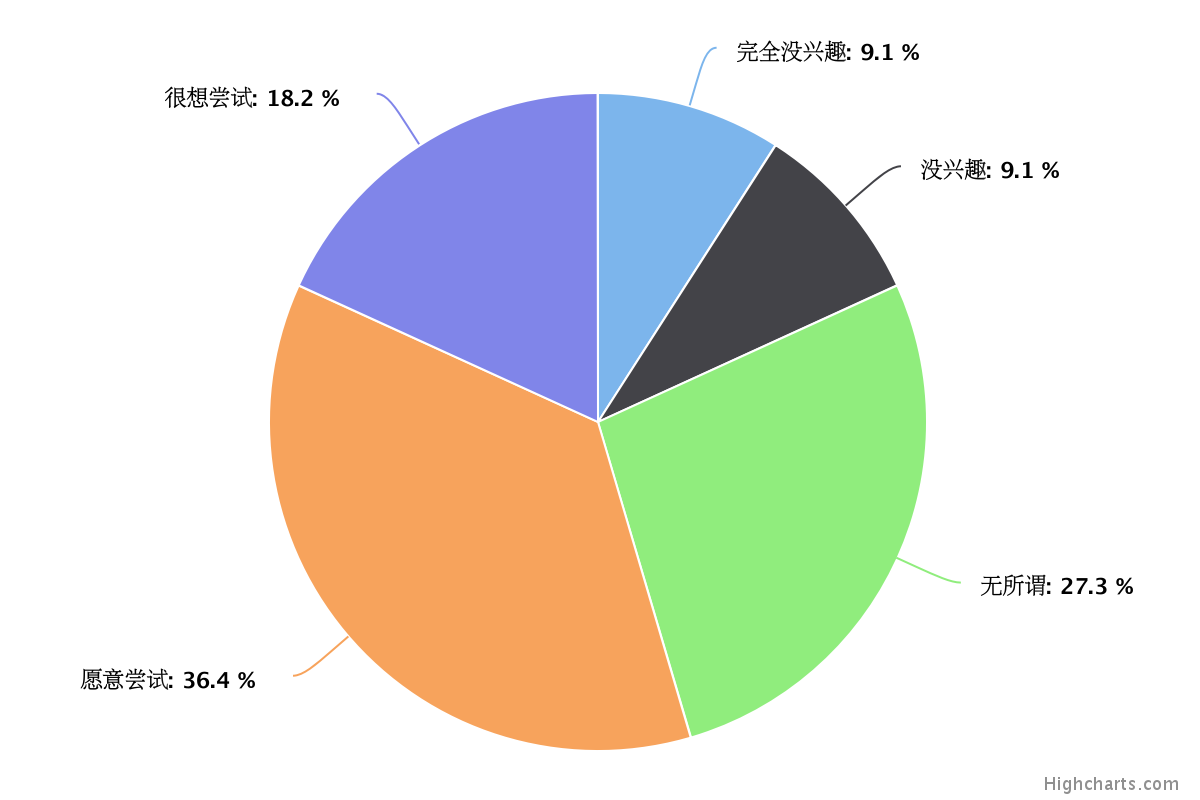
\includegraphics[width=22em]{chart5.png}\\
  \caption{您觉得用手势玩音乐游戏怎么样}\label{2-5}
\end{figure}
\paragraph{}
如果只是提到用手势这种新奇的交互方式的话,出于对VR设备的好奇和新鲜感,大多数用户很乐于去尝试。传统的PC音游交互方式无非就是光标+按键,而光标的操作方式主要就是:鼠标,数位板和触摸屏;按键的操作方式基本就是键盘。
这种平面的二维操作方式已经不能给用户新鲜感。
\paragraph{用户面临的问题}
\begin{figure}[H]
  \begin{minipage}{0.5\linewidth}
    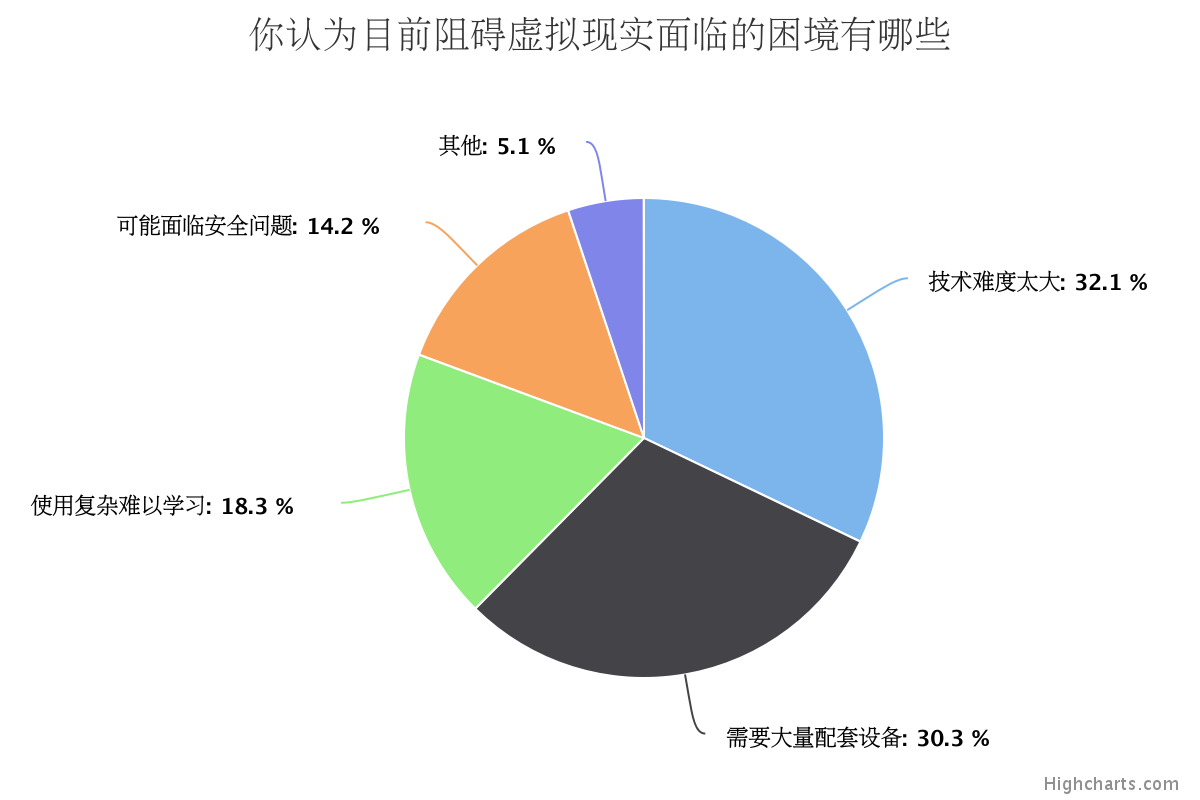
\includegraphics[width=16em]{chart7.png}\\
    \caption{你认为目前阻碍虚拟现实面临的困境有哪些}\label{2-6}
  \end{minipage}
  \begin{minipage}{0.5\linewidth}
    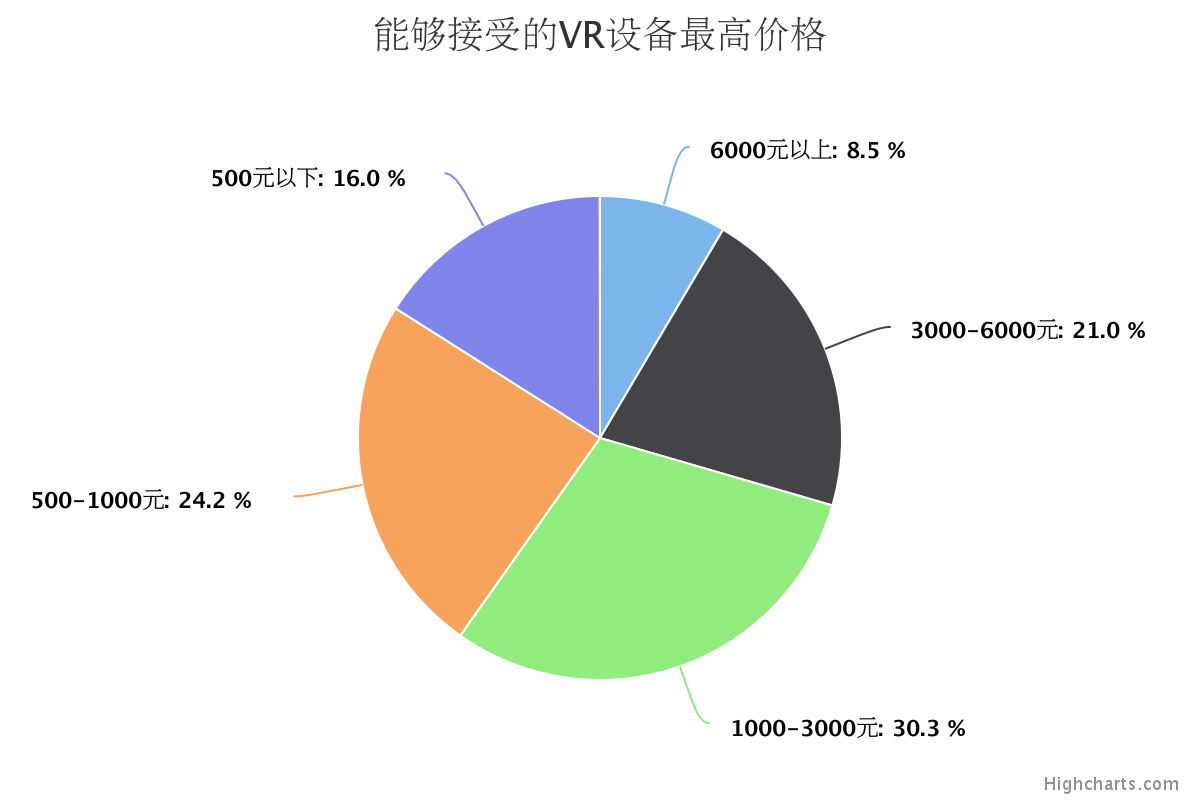
\includegraphics[width=16em]{chart8.png}\\
    \caption{为了喜爱的游戏能接受的VR设备价格}\label{2-7}
  \end{minipage}
\end{figure}
\paragraph{}
可以看到,作为一个新兴的技术,VR包括我们将要使用的手势识别,仍旧面临许多困难,特别是设备价格不够亲民的问题。2016年被称为VR的元年,许多消费级的VR设备在这一年纷纷上市:HTC和steam合作的\textbf{VIVE},FaceBook收购并支持的\textbf{Oculus},Sony配合PlayStation4推出的\textbf{PlayStation VR}.......这些都是几千块钱的集显示和输入于一体的虚拟显示设备,当然也有类似于LeapMtion这种小巧另类的产品存在。400块钱就能让你用更立体、更前卫的方式与电子设备交互,如果能不断提高它的效果,相信也是许多用户可以接受的。
\subsection{玩家分析和同类对比}
\subsubsection{MUG类型概述}
音乐游戏从玩法上有许多种类,虽然业内没有明确的区分,但是从玩家的角度,一般大致分为这么几种。
\begin{description}
  \item[下落式] 模拟钢琴演奏,一般为竖屏,音符从上沿某个轨道下落,至琴键位置时需玩家点击。后来也有音符从中间向四周扩散等方式。
  \item[缩圈式] 俗称“打地鼠”,在屏幕的某个地方会出现一个逐渐缩小(或是其他能看出进度)的图案,当缩小到最佳时机时,玩家点击,将打出符合音乐的节拍。
  \item[其他] 出了上面两大类,还有一些另辟蹊径的音乐游戏,它们也多多少少有借鉴下落式或缩圈式的设计。
\end{description}
无论是哪种模式,音乐游戏的本质,就是让玩家能够按照音乐节拍来进行输入,其中几个很关键的因素就是
\paragraph{判定}玩家按键的准确度,符合节拍的程度
\paragraph{手速}快节拍,高密度的图谱需要一定的手速
\paragraph{读图}熟悉游戏节拍的出现方式,能够快速反应甚至通过肌肉记忆按照节拍打击。\\
\subsubsection{用户群体分析}
\paragraph{}
无论哪种要素,都需要通过不断地训练才能提升。许多人耗费了不少的时间在其中,并且成为了所谓的“大神”;而大多数玩家可能没有足够的时间和耐性成为音乐游戏的“熟练工”,他们自诩为“娱乐党”,不追求完成高难度的谱面,而是享受音乐、享受游戏带来的快乐。
\paragraph{}
要兼顾不同层面的玩家,就要求游戏有一定深度,给玩家提升的空间,同时也要容易上手,有大量适合新手的图谱。许多MUG在这方面已经做得不错了,并且它们也有自己其他闪光的方面
\subsection{同类产品对比}
\paragraph{Deemo}
中文名“古树旋律”,是台湾著名的游戏公司”雷亚“制作的一款下落式移动端音乐游戏。作为一款音乐游戏,Deemo在游戏性上虽然也很好,但只能说是站在了成熟的下落式的肩膀上,并没有太多创新。但是它凭借其独特唯美的画风,和感人的剧情获得了用户的喜爱。
\paragraph{Osu!}
Osu主打的旗号就是免费、自由和玩家互动。游戏本身属于缩圈式,但是它的图谱超过了上亿张,很重要的原因就是它的图谱全部是由玩家自己制作的。可以说Osu!的客户端只是游戏本体的很小一部分,游戏的主要内容大都在其构建的玩家社区中。但是太过社区化的缺陷就在于流失了大量娱乐玩家和新手。作图是一项比较困难的工作,一般只有长时间游戏并有大量作图经历的玩家才能做出好玩的图来,而这些玩家大多又不会制作低于自己水平的图,这就造成了简单图的减少和粗制滥造。另一方面,图谱太多让新手用户难以选择也是让许多新人望而生畏的原因之一。
\paragraph{节奏大师}
又是一款下落式,这款腾讯出品的移动端音乐游戏,依旧没有冲破下落式的束缚。但是它在玩家交互和付费上下了更多的功夫,让它玩起来更像是一个网游,通过出售的人物、道具来降低玩家打图的难度。虽然可能某种程度上让一些音游发烧友唾弃,但却是是一种很好的吸引和黏着用户的方法。
\paragraph{}
与传统音乐游戏相比,MusiCube最大的亮点就在于其革新的交互方式,将输入从原来的二维变成了三维。其次,MusiCube通过图谱编辑器,增加游戏自由度,方便构建游戏社区。
\section{软件设计}
\subsection{架构图}
本软件主要采用Unity3D制作,通过LeapMotion或者键盘鼠标来进行用户交互。软件进入主界面后,可以选择歌曲或是添加歌曲。对每一个歌曲,有两种操作:演出、编辑。每首歌可以有多个难度。
\begin{figure}[H]
  \centering
  % Requires \usepackage{graphicx}
  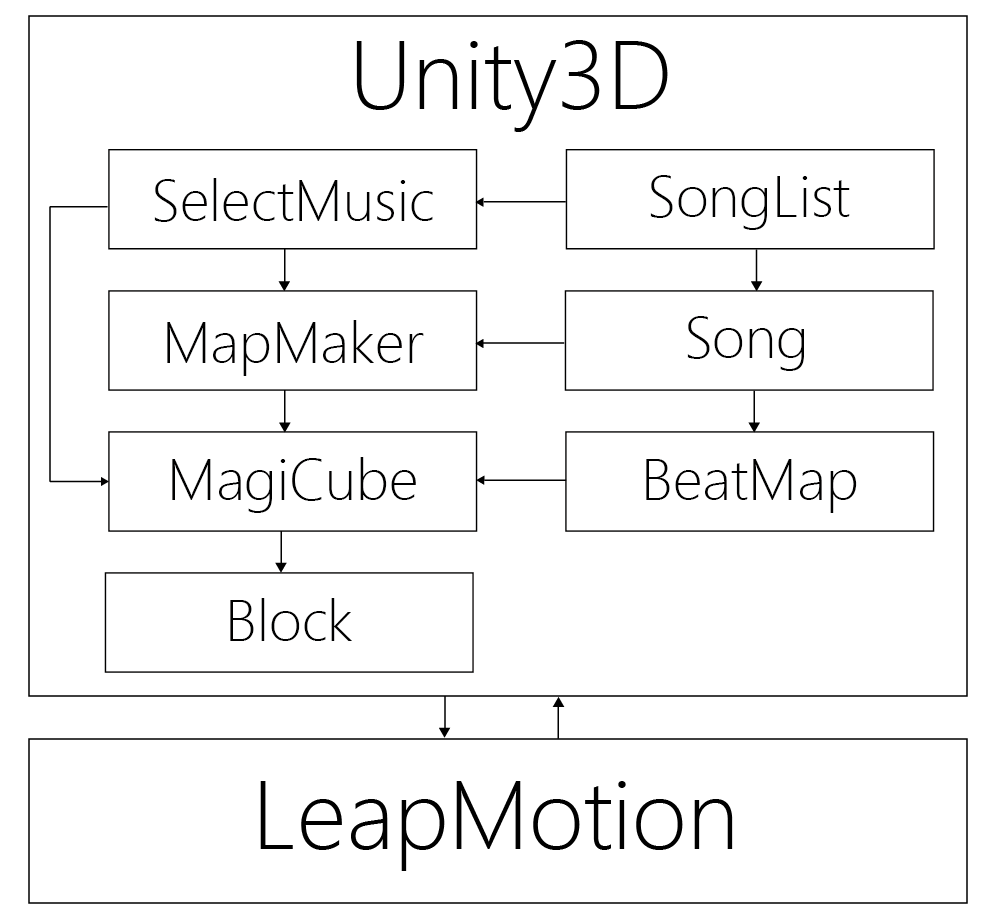
\includegraphics[width=20em]{arc.png}\\
  \caption{}\label{}
\end{figure}
\begin{description}
  \item[Block] 魔方的一个单独方块
  \item[MagiCube] 整个魔方,包含27个Block,提供许多控制接口
  \item[MapMaker] 包含魔方,为编辑图谱提供许多接口,并可以根据BPM(每分钟节拍数)划分时间轴
  \item[SelectMusic] 选歌类,为选歌界面主要元素,可以根据用户输入进入打图或者编辑界面,包含一个SongList
  \item[SongList] 读取预设目录下所有歌曲文件,并为SelectMusic所使用
  \item[Song] 一个Song包含多个BeatMap,即多个歌曲难度
  \item[BeatMap] 一个单独的图谱,是玩家打图的基本单位,主要数据由文件中读取
\end{description}
\paragraph{数据格式}
歌曲和图谱文件放在\textbf{Songs}文件夹内,每一个文件夹是一个单独的\textbf{Song},每一个\textbf{Song}文件夹内有一个\textbf{mci}文件和若干个\textbf{mcb}文件。其中\textbf{mci}文件记录了这首歌曲的一些信息,每个\textbf{mcb}文件则是一个单独的难度,文件头部记录了此难度的信息,接下来是具体的物件信息。
\begin{figure}[H]
  \centering
  % Requires \usepackage{graphicx}
  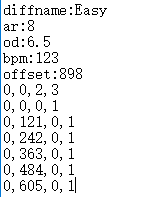
\includegraphics[width=8em]{mci.png}\\
  \caption{}\label{}
\end{figure}
\paragraph{}
数据部分有多行四列,每一行是一个单独的物件,对应着游戏内的一次需要用户操作的音符。而四列从左到右分别为:物件类型编号、时间戳(毫秒)、方块编号、方向编号
\subsection{制作难点}
\paragraph{Unity3D内置音频支持问题}
由于希望能够用户自制图谱,所以游戏需要从外部读取文件(包括音频文件)。但是经过查询文档和测试发现,Unity3D内置的音频支持在Windows平台下,只能从外部读取\textbf{.ogg}格式的文件。
\paragraph{}
现阶段采用的方式是只支持\textbf{.ogg}格式的音频,以后准备使用\textbf{NAudio}库来支持大部分格式的音频文件,并将数据加载进Unity3D内置的音频支持类中。
\paragraph{音频采样率导致计时不准}
由于音频数据等电子数据的特点,它们在时间上不是连续的。如采样率为44100Hz的一个音频文件,其一秒内有44100个采样点,也就是大约每0.023毫秒一个数据。而Unity3D内置的\textbf{AudioSource}类在获取播放时间时,
返回的是按照采样点算出的时间,与真实时间有微小误差,又由于编辑图谱时要对节拍进行划分,按照节拍划分在时间轴上前进、后退。这个误差导致了之前前进、后退的失效。
\paragraph{}
在使用从\textbf{AudioSource}获得的时间前先将其转化为划分好的节拍倍数,也就消除了由于离散采样导致的时间误差问题。
\paragraph{LeapMotion精度问题}
虽然LeapMotion一直吹捧自己的高精度、低延迟,在经过它的驱动Orion升级后,LeapMotion的性能得到了长足的提升,但是经过测试发现它还有不少问题。
\begin{description}
  \item[精度] 虽然精度有待提高,但是对于一个3X3一共27个面的魔方来说,能够在4立方英尺工作的LeapMotion基本足够了
  \item[延迟] 一般音乐游戏的最佳判定在正负20到30毫秒左右,而要使玩家获取较为舒服的游戏体验,游戏帧数可能需要达到240或更高。由于不易测量,我们使用官方提供的参数——最大290帧,也基本满足我们的需求。
\end{description}
\paragraph{UI、模型和动画设计制作}
游戏画面最后的实现效果希望能达到简单优美的效果,在模型的渲染上还要进行调整,计划尝试一些非真实渲染效果,目前的模型可能还需做一些细节上的调整。\\
在动画上面,目前实现的效果并不是十分完美,后期计划加上一些粒子特效,各个动画会根据实际的游戏体验还会进行不同程度的调整。现在还有魔方单层旋转的动画效果还未实现。\\
ui计划使用较扁平的设计风格,具体素材来源根据之后的项目进度再进行确定。
\section{项目进度和规划}
\subsection{当前进度}
\paragraph{}
前半段时间我们把精力放在了底层框架的构建上,主要包括Unity3D开发和一些模型动画的制作。
\paragraph{代码}
实现了游戏中“魔方”类\textbf{MagiCube}的大部分逻辑控制代码,并完成了一个控制它的编辑器类\textbf{MapMaker}。通过这两个类基本可以实现游戏和编辑的两种主要功能。\\
现阶段完成了\textbf{MagiCube}的一种游戏模式,也就是方块的弹出,但是底层接口都已经实现,由于模型动画制作较为复杂所以暂时没有实现其他游戏模式。\\
同时我们还完成了游戏主界面——选歌界面的初始版本,能够完成大部分游戏界面交互的功能,后期会对这个界面进行完善和美化。
\begin{figure}[H]
  \centering
  % Requires \usepackage{graphicx}
  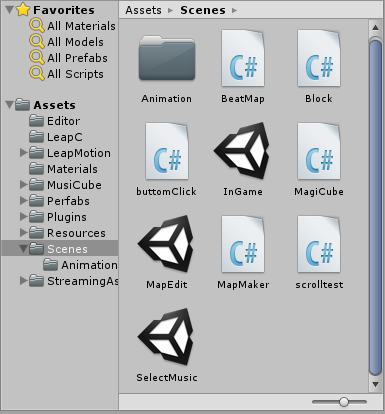
\includegraphics[width=18em]{work.png}\\
  \caption{}\label{}
\end{figure}
\paragraph{模型/动画}
完成了“魔方”的模型和动画制作,动画包括
\begin{enumerate}
  \item 编辑时选择
  \item 编辑时取消选择
  \item 游戏时弹出
  \item 游戏时击打 - Perfect判定
  \item 游戏时击打 - Good判定
  \item 游戏时击打 - Normal判定
  \item 游戏时击打 - Miss判定
  \item 魔方转动前的弹出动画
  \item 魔方转动时的动画
\end{enumerate}
\paragraph{}
游戏中动画的实现是通过代码和动画曲线实现的,可以在Unity3D内灵活调整动画参数,在编辑器和游戏运行时都可以改变动画效果,并提供了单帧播放的接口。
\paragraph{UI}
设计实现了部分UI效果
\begin{enumerate}
	\item 编辑界面中的Note位置和数量提示框
	\item 初始界面的方块膨胀效果
	\item 按钮动画
\end{enumerate}
\begin{figure}[H]
  \centering
  % Requires \usepackage{graphicx}
  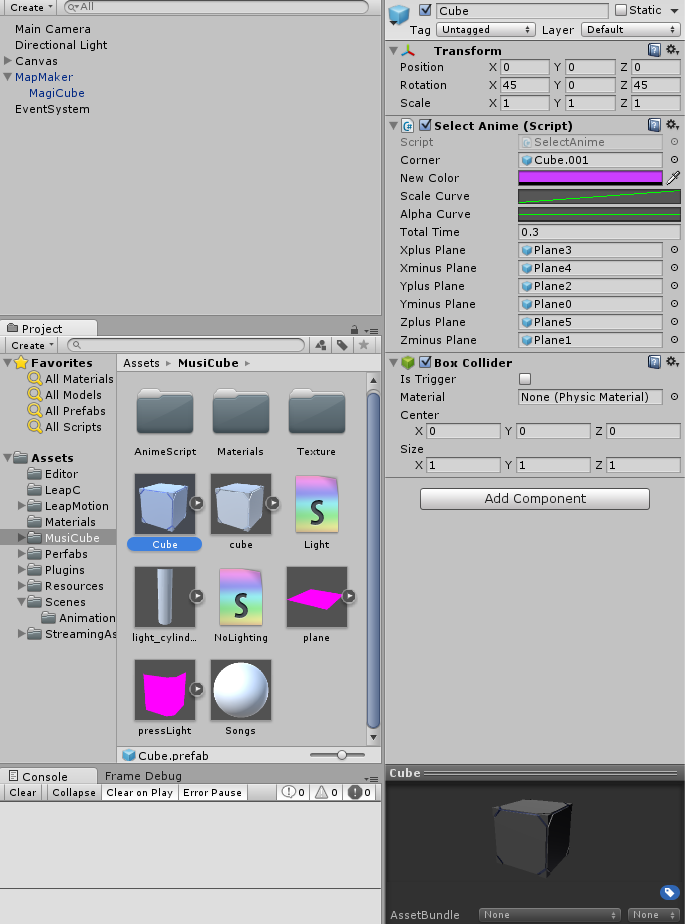
\includegraphics[width=18em]{work1.png}\\
  \caption{}\label{}
\end{figure}
\newpage
\subsection{下阶段计划}
在前半学期的努力下,我们已经搭建好了游戏的底层框架,主要是编辑器和游戏主体“魔方”部分。下一阶段我们将完成学期初的目标。
\begin{enumerate}
  \item 增加滑动一层的游戏模式
  \item 美化选歌界面和编辑界面的UI
  \item 使用NAduio进行音频读取,支持大部分音频格式
  \item 调整缩圈时间和判定时间,改善LeapMotion交互体验
\end{enumerate}
\end{document}
